\documentclass[a4paper, 12pt]{article}

% packages
\usepackage[english]{babel}
\usepackage[T1]{fontenc}
\usepackage[utf8]{inputenc}
\usepackage{csquotes}
\usepackage[backend=biber, style = apa]{biblatex}
\AtEveryCitekey{\clearfield{abstract}}
\usepackage{dsfont}
\usepackage{authblk}
\usepackage{microtype}
\usepackage{amstext}
\usepackage{amssymb}
\usepackage{amsmath}
\usepackage{mathptmx}
\usepackage{setspace}
\usepackage{appendix}
\usepackage{tabularx}
\usepackage{booktabs}
\usepackage{caption}	
\usepackage{pdfpages}
\usepackage[margin = 1in]{geometry}
\captionsetup{singlelinecheck=off,font=small,labelfont=bf}
\usepackage[nolists,tablesfirst,nomarkers]{endfloat}

% commands
\newcommand{\RR}{\raggedright\arraybackslash}
\newcommand{\RL}{\raggedleft\arraybackslash}
\newcommand{\CC}{\centering\arraybackslash}
\setlength{\parindent}{2em}
\setlength{\parskip}{0em}

% directories
\newcommand{\bibdir}{./bib}
\newcommand{\figdir}{../figures}
\newcommand{\tabdir}{../tables}

% bibliography
\addbibresource{\bibdir/csc_research.bib}

% figures/tables
\AtEndDocument{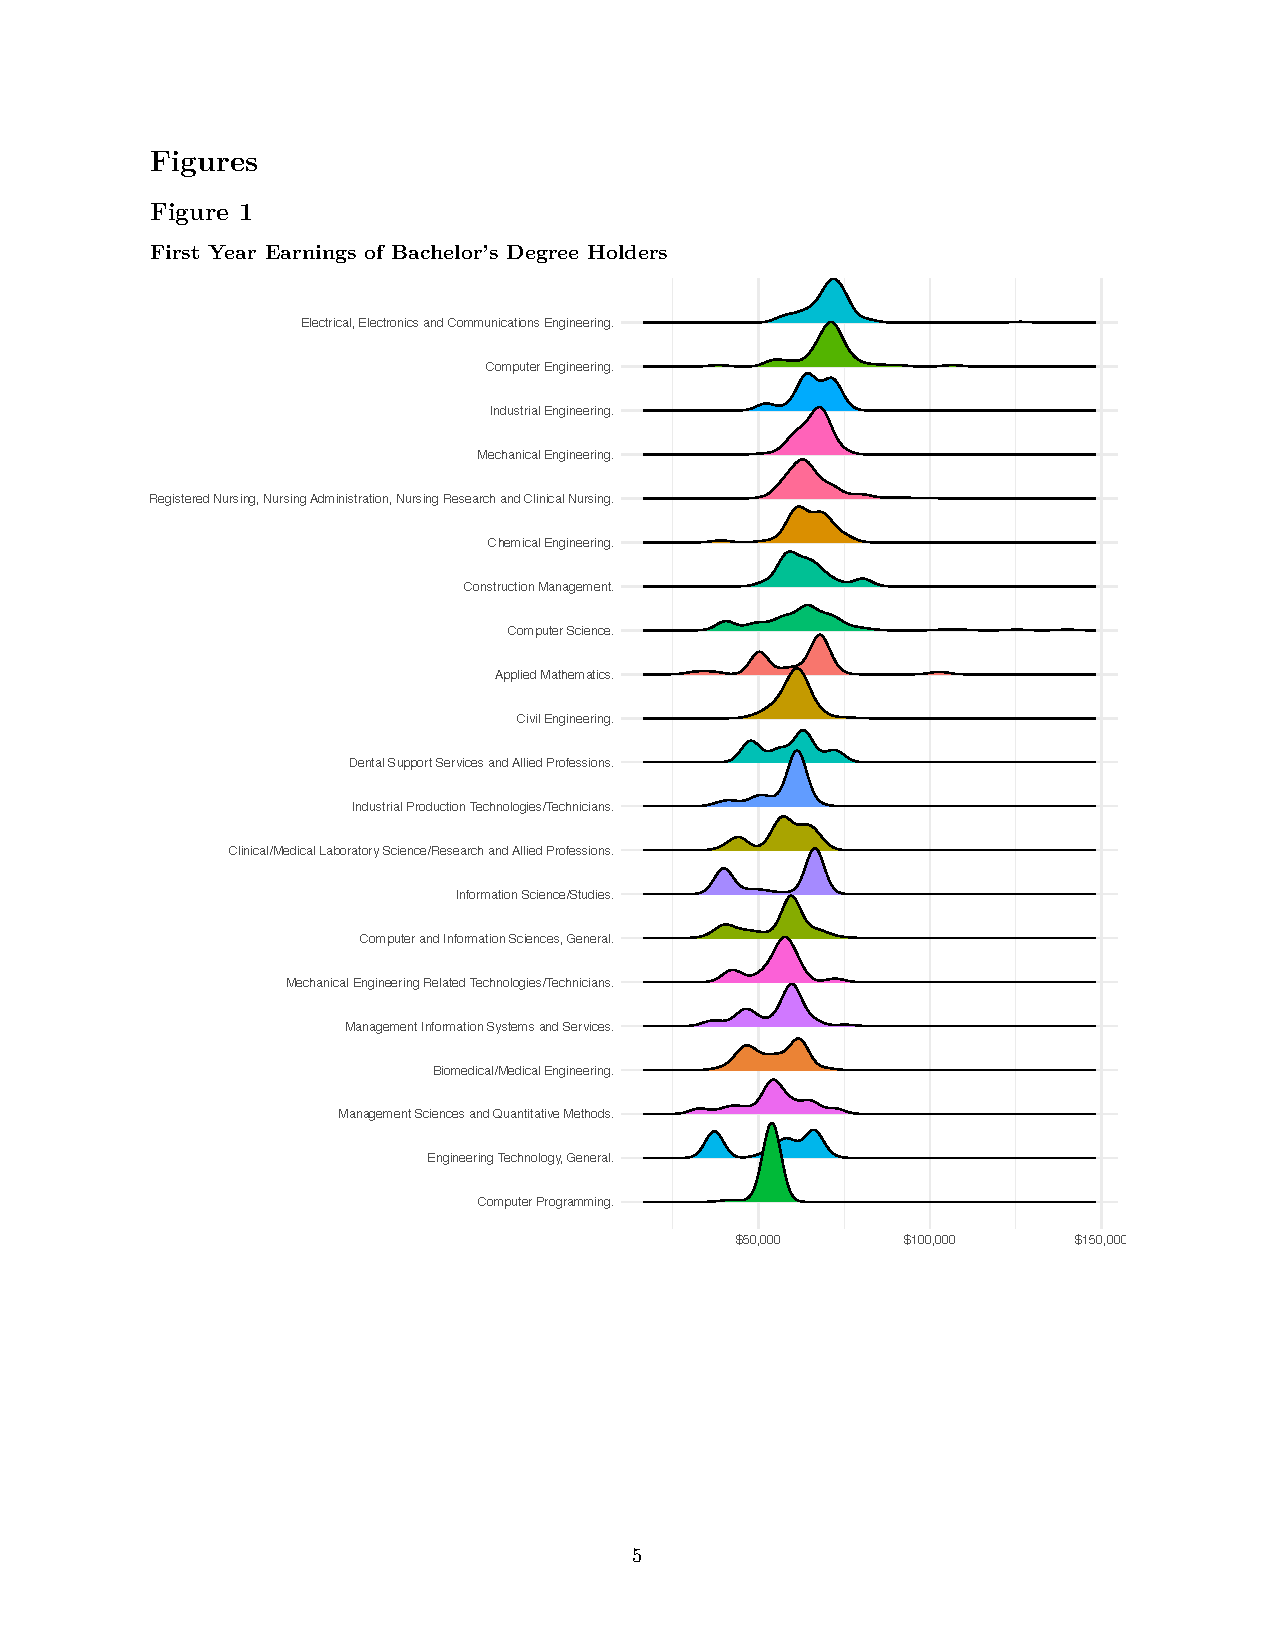
\includepdf[pages=-]{\figdir/tables_figures_references.pdf}}

% author information
\title{Employing Machine-Learning Approaches in Predicting Incomes of Recent College Graduates}
\author[1]{Benjamin Skinner}
\author[2]{Olivia Morales}
\author[3]{William Doyle}
\affil[1, 2]{University of Florida}
\affil[3]{Vanderbilt University}

\date{\today}

\begin{document}

\maketitle

\doublespacing

\begin{center}
\section*{Abstract}
\end{center}

Using a principled machine-learning approach, we predict recent
college graduates' earnings using data from the College
Scorecard. These predictions are estimated using elastic net
regularization and the random forest algorithm, regression-based
methods adept at producing parsimonious statistical models and
reducing bias. Our results support the predictive capabilities of
institutional characteristics like school classification, overall debt
repayment rates and family income on recent graduate earnings. The
results of this project provide critical insight for state/federal
policymakers to orient resources in improving labor market outcomes
for recent graduates.

\vspace{5mm}

keywords: \emph{machine-learning, earnings premiums, market returns to college}

\pagebreak
\section*{Introduction}

Econometric approaches to predicting earnings after graduation are not
uncommon in the higher education literature, as many researchers have
found evidence of higher education's positive return on investment
\parencite{doyle2016educearn, card:1995, Card:1999, Card:2001,
Oreopoulous_Petronijevic_2013}. However, predictive accuracy and
potential researcher bias are particularly of concern in applying
econometric frameworks in research studies. Moreover, many of these
formative studies utilized unique institutional-level data not widely
available to researchers until the launch of the College Scorecard
tool. The publication of the College Scorecard by the U.S. Department
of Education provided a novel opportunity for higher education
scholars to access national institutional/study-level data for future
researcher endeavors. The under-utilization of this resource, along
with the limited capacity of traditional econometric models, prompts
our study to employ machine learning methods to predict college
graduates' earnings from College Scorecard data.

The principal discourse surrounding the purpose of higher education
always centers the increased earnings potential awarded by a college
education. As such, state and federal policymakers hold a vested
interest in directing economic resources most efficiently, to those
programs and institutions pushing out successful graduates and
contributing to local economies (particularly in the public
institutional context). To do this, relevant stakeholders would find
useful information regarding institutional \& program characteristics
that predict a recent graduate's earnings potential. The results of
this study directly address this desire by providing not only
necessary predictions, but predictions with increased accuracy via
machine-learning methodological approaches.

In this project, we use the tools and procedures of data science and
common institutional/program variables available via the College
Scorecard to provide robust predictions of program earnings for recent
college graduates. To estimate program-level earnings using College
Scorecard data, we use data science-based approaches to data analysis,
which are characterized by principled procedures of data cleaning,
model building, and testing. More specifically, we use two machine
learning models---elastic net and random forest---to identify the
strongest predictors and build robust models of program-level income
\parencite{Hastie_etal_2016, Kuhn_Silge_2022}.

Our findings highlight both expected and unexpected predictors of
earnings potential for recent graduates. As anticipated, the type of
degree received (Associate's, Bachelor's, etc.) typically predicts
differential earnings potential after graduation. However, some fields
(particularly those concentrated in the health sciences, did not
produce significantly different results across degree
credentials. Outside of strict levels of prediction, our remaining
models identified surprising positive predictors of earnings
potential, including total outstanding loan balance and median debt 10
years after graduation. Our random forest model also highlighted
several variables in terms of their importance in prediction. These
variables included family income, number of students included in the
three-year cohort default rate and percentage of students making
progress on their federal loan payments two years after graduation.

This work supports future higher education research in two key
ways. First, we offer an example of a principled approach to data
cleaning, model building, and model checking based in procedures
common to data science that we believe could be more widely
incorporated in higher education policy research
\parencite{Kuhn_Silge_2022}. Second, we take full advantage of these
tools and procedures to fit a large number of institutional data
points available through the College Scorecard to increase the
predictive capacity of our models in determining program/institutional
level earnings.

\section*{Literature Review}

\subsection*{Market Returns from Higher Education}

Affirming higher education's economic return to
students holds a steady place in scholarship on colleges and
universities in the U.S. \textcite{Oreopoulous_Petronijevic_2013} take
a comprehensive look at the research available on market returns to
higher education, reviewing 30 years of literature that ultimately
demonstrates an economic advantage and higher earnings potential for
those individuals with a college education. \textcite{hout_2012} dives
deeper into the economic benefits of a college education,
investigating college returns in times of economic instability. During
the Great Recession, there were notable differences in employment
stability and recovery post-recession between college and non-college
graduates \parencite{hout_2012, hout_etal_2011ch}. Results comparing
certain demographic groups pre- and post-Recession affirm this
difference, with those of higher education levels experiencing less
declines in employment \parencite{hoynesetal_2012}.


\textcite{Carnevale_etal_2011}, however, note an important caveat for
this general earnings boost for college graduates: the potential
earnings increase depends on the type of degree/credential earned and
program of study. Higher education scholars have pondered over this
difference by investigating the long-term earnings premiums afforded
by a college education by degree type and even field of
study. \textcite{kimtamborini_2019} examined this question using data
from the Survey of Income and Program Participation from 2004 \&
2008. Across all levels of post-secondary, sub-baccalaureate education
(Associate's, Certificates, etc.), individuals experienced higher
annual and cumulative earnings compared to their high school graduate
counterparts. More noteworthy, however, were the higher earnings
premiums awarded to Associate's degree holders in the physical/health
sciences as compared to Bachelor's degree holders in the
humanities/liberal arts.

\subsection*{History/Use of the College Scorecard}

The College Scorecard initially launched through the work and advocacy
of then-President Obama and the U.S. Department of Education. The
vision of the Scorecard surrounded this novel opportunity for families
to identify the institutions that provided the best labor outcomes for
their students with the least amount of financial burden
\parencite{obama_2013}. While illuminating varied institutional
characteristics when it was first made publicly available in 2015, the
data in the College Scorecard did not generally produce the kind of
impact the Obama administration envisioned and went mostly
underutilized by consumers \parencite{huntington2016search}. The
Scorecard also fell short of providing complete data profiles of
institutional/program characteristics, as large sections of released
data were missing or privacy suppressed due to small program sizes and
concerns over confidentiality.

Despite its shortcomings, the College Scorecard data have been used in
conjunction with standard econometric approaches to evaluate student
responsiveness to the kinds of college choice information provided by
the Scorecard. \textcite{hurwitz_student_2018} employ a DID framework
to show how college decision-making changed among students from
generally well-resourced high schools after the publication of the
Scorecard. While two college program metrics found in the
Scorecard---graduation rates and average costs---produced virtually no
change in SAT score-sending behaviors, the authors did find that
students directed their SAT scores to schools that, on average, had
higher median earnings for graduates. This signals the salience of
future earnings potential to students who are deciding on college and
program. Other researchers have used econometric-based approaches with
Scorecard earnings data in particular institutional and program
contexts \parencite{boland_effect_2021, elu_earnings_2019,
mabel_value_2020, seaman_assessing_2017}.

\subsection*{Machine-Learning Methods in the Academy}

With the growing Scorecard literature, it remains important to
consider the ways common econometric approaches may lead to
misspecified models and unintentional researcher bias when estimating
the relationship between program characteristics and graduate earnings
\parencite{Imbens_2004}. Compared to the standard econometric toolkit,
approaches based in data science and machine learning can improve
estimate quality by following structured procedures and computational
algorithms to build, test, and train models
\parencite{Hastie_etal_2016}. Historically associated with
computational statistics and computer programming methods, tools of
data science and machine learning have been increasingly used among
higher education researchers to provide principled estimates,
including those that would not otherwise be possible with standard
econometric methods \parencite{skinner2021civic, aulck2017predicting,
savvas_etal_2021, Zeineddine_2021}.

Random forest models, in particular, have been featured in recent
higher education studies as an improvement mechanism for prediction
and identification of variable importance in statistical models. In
their study of predicting academic success and major,
\textcite{beaulacrosenthal_2019} determined that the random forest
models utilized consistently outperformed the comparable logistic
regression models in their predictive capacities. Elastic net
regularization (as a tool to improve the generalization of regression
models) is less common in the education literature, but is supported
by various writings in scholarship on statistical methods. Originally
proposed by \textcite{zouhastie_2005} as a boost to the use of solely
LASSO/ridge regression penalties in variable selection, it now enjoys
a regular presence in statistics and computation journals
\parencite{zouzhang_2009, lilin_2010}.

Our project situates itself uniquely in the larger higher education
literature by marrying relatively novel statistical/machine learning
methods with an underutilized, rich data resource to model salient
predictions of earnings potential for recent college graduates.

\section*{Policy Context}

While the national trends of state appropriations for higher education
have improved considerably in the last ten years, funding for
U.S. colleges/universities has not fully recovered in the aftermath of
the Great Recession \parencite{shef_2021}. Local financing mechanisms
have tried to address the devastation of the Recession (particularly
in the community college context). However, differences in local
funding contexts have prevented gaining much lost ground in this area
nationwide \parencite{dowdgrant_2006, cap_2020}.

As such, policymakers invested in the advancement of their state's
higher education institutions rely on the empirical evidence provided
by higher education researchers to advocate for increases in
appropriation allocations \parencite{terenzini_1996}. In a
contemporary example, members of the Florida House of Representatives
Higher Education Appropriations subcommittee utilized a research
report detailing the shortage of nurses in the state as a result of
the COVID-19 pandemic. To address this issue, recommendations were put
forth to expand the capacity of existing nursing education programs
across Florida \parencite{floridahouse_2022, workforce_2021}.

The reality of the state of higher education funding
necessitates policy making in anticipation of economic/workforce
needs. Our study fits neatly into this narrative by providing
predictive earnings potential that could inform policy making,
supporting calls for program/degree expansions with informed
predictions that fulfill state/local demands.

\section*{Methodology and Model Specification}

To estimate program-level earnings using College Scorecard data, we
use data science-based approaches to data analysis, which are
characterized by principled procedures of data cleaning, model
building, and testing. More specifically, we use two machine learning
models---elastic net and random forest---to identify the strongest
predictors and build robust models of program-level income
\parencite{Hastie_etal_2016, Kuhn_Silge_2022}.

For our models, we use two regression-based, machine-learning methods:
elastic net and random forest. Elastic net regularization combines
LASSO and ridge regression penalties to remove non-predictive
coefficients and shrink correlated parameters towards each
other. Random forest regression models average results from a large
number of decision trees fit to a random subset of observations and
covariates \parencite{Hastie_etal_2016}. Below is the regression model
defined for both methods:

\[y_i = \alpha + c_i\gamma + \epsilon_i\]


\noindent where \newline $y_i$ is the outcome variable (median
earnings of graduates one year after graduation)\newline $\alpha$ is
the intercept \newline $c_i$ is a vector of covariates \newline
$\gamma$ is a vector of coefficients for those covariates \newline
$\epsilon_i$ is an error term

These models are particularly useful in our project, as they provide
two key benefits. First, they offer principled predictor selection
from a large set of possible determinants of earnings. Second, they
also support the identification of non-linear relationships between
predictors, which means our predictions are not dependent on a
researcher-established functional form in the model. Using these two
modeling approaches we identify variables in the Scorecard data set
that are highly predictive indicators of our dependent variable of
interest: median earnings from graduates of the program after one
year.

\subsection*{The Tidymodels Philosophy}

Our approach to data processing and model selection is informed by
\textcite{Kuhn_Silge_2022}'s Tidymodels framework. This framework
explains the normative process of data manipulation to model selection
to performance evaluation as step-by-step instructions of a recipe. In
our project, this begins by performing a pipeline of pre-processing
work on our merged College Scorecard/ACS dataset. This pipeline
delineates the steps or functions in R that are (1) dropping privacy
suppressed/missing data elements, (2) recoding categorical data to
dummy-coded indicator variables, and (3) removing zero variance/highly
correlated predictors. Once completed, the dataset will be associated
with a ``recipe'' object in our RStudio environment. 

Next, we partition our original dataset into two subsets: a training
set for model building and a test set for model performance
evaluation.  We then perform k-fold cross validation on the training
set specifically, recursively splitting the training set into 20
separate data sets to train and average across models. After deciding
upon the best model (using RMSE as our performance metric), we use it
to predict program-level earnings using the held-out testing
data. These procedures (training/test sets and cross-validation) help
mitigate issues of overfitting that can bias results too closely to
particular samples.

Model selection is facilitated by a tuning grid, defined by the
researcher to experiment with tuning the model's hyperparameters. Our
hyperparameters of interest in performing elastic net regularization
are penalty and mixture; the tuning grid constructed will test various
models (built over resampled data sets) with different value
combinations (between 0 and 1) for both the penalty and mixture
arguments. The values most adept at producing the model with the
lowest RMSE is identified for final model selection. The function
select\_best() will ease this process, and finalize\_model() will marry
both the random forest algorithm /& best-performing hyperparameters
for use on the testing data set.

Our random forest model selection works in a similiar fashion, tuning
the min\_n (minimum node size) and mtry (number of sampled covariates
in a tree) arguments over an integer-defined grid. This integer
indicates how many sets of parameters should be tested over the
resamples of the data achieved via cross-validation. With slight
changes to the engine (software) used for the model, we can perform
the same tuning process and use select\_best() to identify the optimal
hyperparameters for our model. Utilizing the finalize\_model() function
will help us arrive to our principal model of variable importance.

The entire process from recipe to model selection is defined in a
workflow object in our RStudio environment. This workflow object
instructs RStudio to perform the aforementioned steps (data recoding,
model fitting with regression formula, hyperparameter tuning)
sequentially to arrive at the best-performing models for each
regression-based method.


\section*{Data}

Data for this project originate from two specific sources: the College
Scorecard and American Community Survey. We focus on the most recent
2019-2020 College Scorecard data. In addition to our key outcome
variable of interest, median earnings for college graduates one year
after graduation, we take advantage of the large number of variables
available in the College Scorecard data set. These include over 2,000
variables featuring institutional characteristics and program-level
data for 6,700 accredited institutions in the U.S., including type of
institution, degrees awarded, and the number of loan borrowers among
many others.

Using unique county FIPS codes, we match each higher education
institution with county-level data from the ACS. To align with the
latest Scorecard data, we use 2019 ACS estimates. At this time, we
include the percentage of adults who have attained a bachelor's degree
or higher; the percentage of homeowners; percentages of adults in the
labor force; and median household income. Because a significant amount
of individual student information in the Scorecard data is suppressed
for privacy reasons, including county-level data from the ACS allows
us to recover some information that is useful for predicting earnings
of recent graduates.

\section*{Findings}

Across Figures 1-3, we show median first year earnings for a selection
of programs at three degree levels: Bachelors, associate and
certificate/diploma. Across the figures, we see generally greater
earnings potential for Bachelors degree holders compared to associate
degree and certificate/diploma holders in similar fields of study. For
example, those who earn a Bachelors degree in computer programming
earn just over \$50,000 in their first year compared to computer
programmers with an associates degree or those with a certificate in
computer systems networking and telecommunications who earn closer to
\$30,000. On the other hand, there are some fields that do not show
much difference in median first year earnings. As an example, nurses
with an associate degree earn about the same in the first year, about
\$60,000, as those with a Bachelors degree.

Figure 4 shows predictor estimates from the elastic net model (see
Table 1 for a concordance of variable names with their
descriptions). The length of the bars represent the strength of the
predictive power of the variable, with the color of the bars
representing the direction of the association. While we identify some
variables typically assumed to be positive predictors of graduate
income like type of school, type of degree/credential, we also find
some unexpected positive and negative predictors of first year
earnings, like outstanding federal loan balance and median debt for
graduated students.

Figure 5 shows the most important variables from our random forest
regression model, meaning those variables that, across all decision
trees, tend to be the most predictive of median first year
earnings. As with our elastic net model results, we see a similar
emphasis on the importance of type of degree credential, specifically
certificate/diploma and Bachelor's degrees. We also see the importance
of median family income and average family income for those students
who are considered independents. Less expected are the comparative
importance---compared to many thousand predictors---of three-year
cohort default rates and the percentage of students making
satisfactory academic progress by completing their coursework within
eight years at the original institution.

\section*{Implications/Conclusions}

Data science and machine learning approaches in combination with
domain knowledge hold incredible possibilities in determining the
college and program-level features most predictive of key student
outcomes such as first year earnings. It is evident that the
integration of machine learning into higher education research
methods/practice has already begun, and this project adds to this body
of work.

While the technical nature of data science and machine learning
approaches to prediction may sometimes seem removed from the higher
education policy landscape at large, this study, at its foundation,
cares about the material outcomes for students who invest their money
and time in their educational futures. We employ our principled data
scientific approach so that we might identify the strongest predictors
of college graduates' incomes without introducing bias through our
variable selection and modeling choices. Our ultimate goal with this
work is to provide information on the predictors of strong programs
that will inform policy and practice that amplifies positive student
earnings potential.

\pagebreak
\setstretch{1}
\setlength\bibitemsep{0.5\baselineskip} 
\printbibliography
\end{document}
